\section{Frontend}
\subsection{Technologies and libraries}
\subsubsection{NextJS}
NextJS is an open-source\textsubscript{\textbf{G}} React framework\textsubscript{\textbf{G}} created by Vercel. It supports TypeScript, static generation\textsubscript{\textbf{G}} and server-side rendering\textsubscript{\textbf{G}} which improves the site's search engine optimization. It also supports dynamic routing of pages.
\begin{itemize}
  \item \textbf{Used Version: 10.2}
  \item \textbf{Link: \url{https://nextjs.org/}}
\end{itemize}
\subsubsection{React}
React is an open-source\textsubscript{\textbf{G}}, frontend, Javascript library for building user interfaces, maintained by Facebook. It's component based and it supports TypeScript. Since is made for single-page development additional libraries are required for routing.
\begin{itemize}
  \item \textbf{Used Version: 17.0.3}
  \item \textbf{Link: \url{https://reactjs.org/}}
\end{itemize}
\subsubsection{Chakra UI}
Chakra UI is a React component library made with TypeScript and NextJS in mind. It is accessible and flexible, makes the styling fast and easy.
\begin{itemize}
  \item \textbf{Used Version: 1.6.1}
  \item \textbf{Link: \url{https://chakra-ui.com/}}
\end{itemize}
\subsubsection{NextAuth}
NextAuth.js is a complete open source authentication solution for Next.js applications. It is designed from the ground up to support Next.js and Serverless.
\begin{itemize}
  \item \textbf{Used Version: 3.14.8}
  \item \textbf{Link: \url{https://next-auth.js.org/}}
\end{itemize}
\subsubsection{Swiper}
Swiper is a React componenent that render a touch slider with hardware accelerated transitions.
\begin{itemize}
  \item \textbf{Used Version: 6.7.0}
  \item \textbf{Link: \url{https://swiperjs.com/}}
\end{itemize}
\subsubsection{Cookies}
Cookies is a node.js module for getting and setting HTTP(S) cookies.
\begin{itemize}
  \item \textbf{Used Version: 0.8.0}
  \item \textbf{Link: \url{https://www.npmjs.com/package/cookies}}
\end{itemize}
\subsubsection{Jest}
Jest is a JavaScript testing framework designed to ensure correctness of any JavaScript codebase.
\begin{itemize}
  \item \textbf{Used Version: 27.0.6}
  \item \textbf{Link: \url{https://jestjs.io/docs/getting-started}}
\end{itemize}
\subsection{General description}
The frontend\textsubscript{\textbf{G}} structure has three macro categories that explains its works:
\begin{itemize}
  \item data fetching
\end{itemize}




is based on using the npm utilities-techsweave package produced by the backend, containing the interfaces and services useful for rendering the user interface. The interfaces of the microservices are imported by the "Models" file, while the methods made available by the microservices are imported by the "Services" file. These methods allow to call the lambda functions present within the backend to obtain the results necessary for the functioning of the user interface. To render the pages of the platform, the best practices of React and Next.js are followed. The pages are composed through the use of components, HTML snippets\textsubscript{\textbf{G}} that reproduces a specific part of the page itself.

\begin{figure}[!ht]
  \caption{Profile page navbar}
  \vspace{10px}
  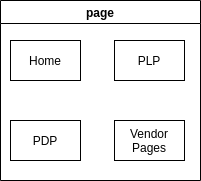
\includegraphics[scale=0.3]{../../../../Images/Diagrammi/maintainerManual/FEgraph.png}
  \centering
\end{figure}


\subsection{Examples of functioning}
\subsubsection{Use of a function}
The scan of the products in the database will be returned when calling the scanAsync method on an instance of the product class. These products will be passed to the frontend components to render the page and display the data taken from the database.
\subsubsection{Rendering of a page}
To render the detail page of a product, by using the getStaticProps function will be returned the data with the necessary product details. The various components are then inserted into the HTML code to produce the page:
\begin{itemize}
  \item \textbf{Layout}, containing the general style of the page including header, footer and navbar;
  \item \textbf{ProductDetail}, to render product details through images and texts;
  \item \textbf{RelatedProduct}, creates a list of products with the same category of the one currently displayed;
  \item \textbf{ProductInfo}, creates a list of products specifications;
  \item \textbf{AddToCart}, displays a button to add the currently displayed product in the cart.
\end{itemize}

